\tikzset{word ladder/.style={
  matrix of nodes
  , execute at empty cell={\node[draw=gray,text=gray,fill=white]{0};}
  , nodes in empty cells=false
  , nodes={shape=rectangle, draw=none,fill=none,text=black,minimum width=0.6cm,minimum height=0.35cm,outer sep=0pt,align=center,inner sep=0pt,font=\small}
  , row sep={0.35cm,between origins}
  , column sep={0.6cm,between origins}
},
}

\tikzset{spacehash board/.style={
  matrix of nodes
  , execute at empty cell={\node[draw=gray,text=gray,fill=white]{ };}
  , nodes in empty cells=false
  , nodes={draw=gray,fill=ocre,text=gray,text depth=0.5ex,text height=2ex,text width=1em,outer sep=0pt,align=center,inner sep=0pt}
  , row sep={#1,between origins}
  , column sep={#1,between origins}
},
}

\tikzset{noughtsone board/.style={
  matrix of nodes
  , execute at empty cell={\node[draw=gray,text=gray,fill=white]{0};}
  , nodes in empty cells=false
  , nodes={draw=gray,fill=ocre,text=gray,minimum width=#1,minimum height=#1,outer sep=0pt,align=center,inner sep=0pt}
  , row sep={#1,between origins}
  , column sep={#1,between origins}
},
  noughtsone board/.default=0.5cm
}

\tikzset{twocolour board/.style={
  matrix of nodes
  , execute at empty cell={\node[text=white,fill=white]{+};}
  , nodes in empty cells=false
  , nodes={draw=gray,fill=ocre,minimum width=#1,minimum height=#1,outer sep=0pt,align=center,inner sep=0pt,font=\tiny}
  , text=ocre
  , row sep={#1,between origins}
  , column sep={#1,between origins}
},
  twocolour board/.default=0.5cm
}
\tikzset{twocolour board/.style={
  matrix of nodes
  , execute at empty cell={\node[text=white,fill=white]{+};}
  , nodes in empty cells=false
  , nodes={draw=gray,fill=ocre,minimum width=#1,minimum height=#1,outer sep=0pt,align=center,inner sep=0pt,font=\tiny}
  , text=ocre
  , row sep={#1,between origins}
  , column sep={#1,between origins}
},
  twocolour board/.default=0.5cm
}

%% Candy Crush-style games, colour & label
\tikzset{crushstyle board/.style={
  matrix of nodes
  , nodes={draw=gray,fill=ocre,minimum width=#1,minimum height=#1,outer sep=0pt,align=center,inner sep=0pt,font=\tiny}
  , text=ocre
  , row sep={#1,between origins}
  , column sep={#1,between origins}
},
  crushstyle board/.default=0.5cm
}

%% WaTor-style games, colour & label
\tikzset{watorstyle board/.style={
  matrix of nodes
  , nodes={fill=cyan,minimum width=#1,minimum height=#1,outer sep=0pt,align=center,inner sep=0pt,font=\tiny}
  , text=black
  , row sep={#1,between origins}
  , column sep={#1,between origins}
},
  watorstyle board/.default=0.25cm
}

%% 8-tile style
\tikzset{eighttilestyle board/.style={
  matrix of nodes, ampersand replacement={\&}
  , execute at empty cell={\node[draw=gray,text=gray,fill=gray]{0};}
  , nodes={fill=gray,minimum width=#1,minimum height=#1,outer sep=0pt,align=center,inner sep=0pt,font=\tiny}
  , text=ocre
  , row sep={#1,between origins}
  , column sep={#1,between origins}
},
  eighttilestyle board/.default=0.25cm
}

\tikzset{sixelstyle/.style={
  matrix of nodes, ampersand replacement={\&}
  , nodes={draw=black,fill=gray,text=gray
     %,minimum height=1pt, minimum width=1pt
     %,row sep=1pt, column sep=1pt
}
},
   sixelstyle/.default=0.3em
}

\tikzset{sepsixstyle/.style={
  matrix of nodes, ampersand replacement={\&}
  , nodes={draw=white,fill=gray,text=gray,
     minimum height=1pt, minimum width=1pt,
     row sep=1pt, column sep=1pt}
},
   sixelstyle/.default=0.3em
}


\nsection{Teletext}

In the early 1970s, Phillips Labs began work on transmitting digital
information across the television network. The aim was to
provide up-to-date news and weather information via a television set. 
This system was trialled first by the BBC in a system that eventually became
known as ``Ceefax'' and then on other independant British terrestrial stations as ``Oracle''.
A very similar system was implemented on the BBC microcomputer, known as {\it Mode 7}.
\begin{figure}[ht]
\centering{
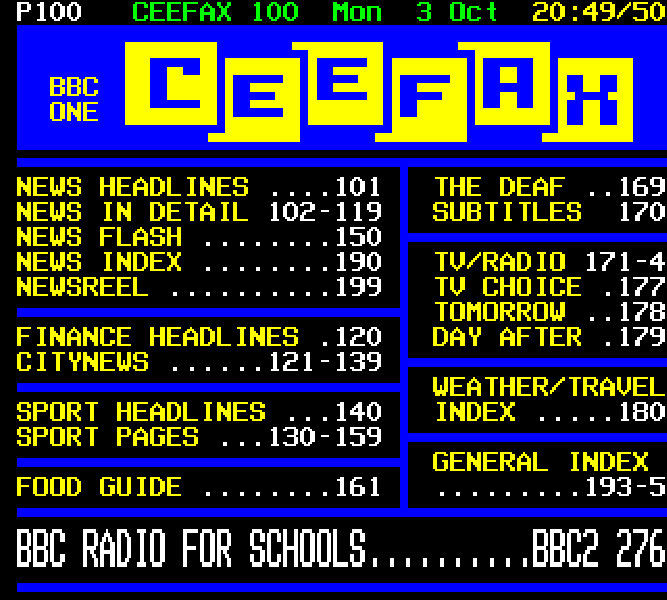
\includegraphics{../Pictures/teletext100.pdf}
}
\caption{An example Ceefax page circa 1983. Taken from {\tt http://teletext.mb21.co.uk/gallery/ceefax/main1.shtml}}
\label{fig:tt100}
\end{figure}
An example of such a Ceefax screen is shown in Figure~\ref{fig:tt100}.

This project, inspired by such teletext systems, will allow a $40 \times 25$ ($1000$) character
file to be rendered to the screen, using similar control codes. However, some control
codes are not implemented, including those to do with flashing or hidden text, and transparent backgrounds. In particular, our definition of the {\it double height} control code differs from that of
the traditional one.

\subsection*{The Control Codes}

This section is based to a large extent to Richard Russell's description of
Mode 7 on the BBC Micro:
\verb^http://www.bbcbasic.co.uk/tccgen/manual/tcgen2.html^.

\begin{table}
\begin{tabular}{|c|c|c|c|c|c|c|c|c|}\hline
   &0x8            & 0x9               & 0xA&0xB&0xC& 0xD         &0xE& 0xF         \\
 0 &Unused/Reserved&Unused/Reserved    &    & 0 & @ & P           & - & p           \\
 1 &Red Alphanumeric       &Red Graphics       & !  & 1 & A & Q           & a & q           \\
 2 &Green Alphanumeric     &Green Graphics     & "  & 2 & B & R           & b & r           \\
 3 &Yellow Alphanumeric    &Yellow Graphics    & $\pounds$  & 3 & C & S           & c & s           \\
 4 &Blue   Alphanumeric    &Blue   Graphics    & \$ & 4 & D & T           & d & t           \\
 5 &Magenta Alphanumeric   &Magenta Graphics   & \% & 5 & E & U           & e & u           \\
 6 &Cyan Alphanumeric      &Cyan Graphics      & \& & 6 & F & V           & f & v           \\
 7 &White Alphanumeric     &White Graphics     &  ' & 7 & G & W           & g & w           \\
 8 &Unused/Reserved&Unused/Reserved    &  ( & 8 & H & X           & h & x           \\
 9 &Unused/Reserved&Contiguous Graphics&  ) & 9 & I & Y           & i & y           \\
 A &Unused/Reserved&Separated Graphics &  * & : & J & Z           & j & z           \\
 B &Unused/Reserved&Unused/Reserved    &  + & ; & K & $\leftarrow$& k &$\sfrac{1}{4}$\\
 C &Single Height  &Black Background   &  , & < & L &$\sfrac{1}{2}$& l & $||$           \\
 D &Double Height  &New Background     &  - & = & M &$\rightarrow$ & m &$\sfrac{3}{4}$\\
 E &Unused/Reserved&Hold Graphics      &  . & > & N & $\uparrow$  & n &$\div$    \\
 F &Unused/Reserved&Release Graphics   &  / & ? & O & \#           & o & \textblock           \\ \hline
\end{tabular}
\caption{The control codes and characters for alphanumeric mode. Note here (because we're using white paper) foreground is shown in black and background in white. On a teletext screen we use white on a black background.}
\label{tab:normgraph}
\end{table}

\begin{table}
\begin{tabular}{|c|c|c|c|c|c|c|c|c|}\hline
   &0x8            & 0x9               		& 0xA&0xB&0xC& 0xD         &0xE& 0xF         \\
 0 &Unused/Reserved&Unused/Reserved    		& \sixel{\bb}{\bb}{\bb}{\bb}{\bb}{\bb} & \sixel{\bb}{\bb}{\bb}{\bb}{\ff}{\bb} & @ & P           & \sixel{\bb}{\bb}{\bb}{\bb}{\bb}{\ff} & \sixel{\bb}{\bb}{\bb}{\bb}{\ff}{\ff}\\
 1 &Red Alphanumeric       &Red Graphics	& \sixel{\ff}{\bb}{\bb}{\bb}{\bb}{\bb} & \sixel{\ff}{\bb}{\bb}{\bb}{\ff}{\bb} & A & Q           & \sixel{\ff}{\bb}{\bb}{\bb}{\bb}{\ff} & \sixel{\ff}{\bb}{\bb}{\bb}{\ff}{\ff}\\
 2 &Green Alphanumeric     &Green Graphics	& \sixel{\bb}{\ff}{\bb}{\bb}{\bb}{\bb} & \sixel{\bb}{\ff}{\bb}{\bb}{\ff}{\bb} & B & R           & \sixel{\bb}{\ff}{\bb}{\bb}{\bb}{\ff} & \sixel{\bb}{\ff}{\bb}{\bb}{\ff}{\ff}\\
 3 &Yellow Alphanumeric    &Yellow Graphics	& \sixel{\ff}{\ff}{\bb}{\bb}{\bb}{\bb} & \sixel{\ff}{\ff}{\bb}{\bb}{\ff}{\bb} & C & S           & \sixel{\ff}{\ff}{\bb}{\bb}{\bb}{\ff} & \sixel{\ff}{\ff}{\bb}{\bb}{\ff}{\ff}\\
 4 &Blue   Alphanumeric    &Blue   Graphics	& \sixel{\bb}{\bb}{\ff}{\bb}{\bb}{\bb} & \sixel{\bb}{\bb}{\ff}{\bb}{\ff}{\bb} & D & T           & \sixel{\bb}{\bb}{\ff}{\bb}{\bb}{\ff} & \sixel{\bb}{\bb}{\ff}{\bb}{\ff}{\ff}\\
 5 &Magenta Alphanumeric   &Magenta Graphics	& \sixel{\ff}{\bb}{\ff}{\bb}{\bb}{\bb} & \sixel{\ff}{\bb}{\ff}{\bb}{\ff}{\bb} & E & U           & \sixel{\ff}{\bb}{\ff}{\bb}{\bb}{\ff} & \sixel{\ff}{\bb}{\ff}{\bb}{\ff}{\ff}\\
 6 &Cyan Alphanumeric      &Cyan Graphics	& \sixel{\bb}{\ff}{\ff}{\bb}{\bb}{\bb} & \sixel{\bb}{\ff}{\ff}{\bb}{\ff}{\bb} & F & V           & \sixel{\bb}{\ff}{\ff}{\bb}{\bb}{\ff} & \sixel{\bb}{\ff}{\ff}{\bb}{\ff}{\ff}\\
 7 &White Alphanumeric     &White Graphics	& \sixel{\ff}{\ff}{\ff}{\bb}{\bb}{\bb} & \sixel{\ff}{\ff}{\ff}{\bb}{\ff}{\bb} & G & W           & \sixel{\ff}{\ff}{\ff}{\bb}{\bb}{\ff} & \sixel{\ff}{\ff}{\ff}{\bb}{\ff}{\ff}\\
 8 &Unused/Reserved&Unused/Reserved		& \sixel{\bb}{\bb}{\bb}{\ff}{\bb}{\bb} & \sixel{\bb}{\bb}{\bb}{\ff}{\ff}{\bb} & H & X           & \sixel{\bb}{\bb}{\bb}{\ff}{\bb}{\ff} & \sixel{\bb}{\bb}{\bb}{\ff}{\ff}{\ff}\\
 9 &Unused/Reserved&Contiguous Graphics		& \sixel{\ff}{\bb}{\bb}{\ff}{\bb}{\bb} & \sixel{\ff}{\bb}{\bb}{\ff}{\ff}{\bb} & I & Y           & \sixel{\ff}{\bb}{\bb}{\ff}{\bb}{\ff} & \sixel{\ff}{\bb}{\bb}{\ff}{\ff}{\ff}\\
 A &Unused/Reserved&Separated Graphics		& \sixel{\bb}{\ff}{\bb}{\ff}{\bb}{\bb} & \sixel{\bb}{\ff}{\bb}{\ff}{\ff}{\bb} & J & Z           & \sixel{\bb}{\ff}{\bb}{\ff}{\bb}{\ff} & \sixel{\bb}{\ff}{\bb}{\ff}{\ff}{\ff}\\
 B &Unused/Reserved&Unused/Reserved		& \sixel{\ff}{\ff}{\bb}{\ff}{\bb}{\bb} & \sixel{\ff}{\ff}{\bb}{\ff}{\ff}{\bb} & K & $\leftarrow$& \sixel{\ff}{\ff}{\bb}{\ff}{\bb}{\ff} & \sixel{\ff}{\ff}{\bb}{\ff}{\ff}{\ff}\\
 C &Single Height  &Black Background		& \sixel{\bb}{\bb}{\ff}{\ff}{\bb}{\bb} & \sixel{\bb}{\bb}{\ff}{\ff}{\ff}{\bb} & L &$\sfrac{1}{2}$& \sixel{\bb}{\bb}{\ff}{\ff}{\bb}{\ff} & \sixel{\bb}{\bb}{\ff}{\ff}{\ff}{\ff}\\
 D &Double Height  &New Background		& \sixel{\ff}{\bb}{\ff}{\ff}{\bb}{\bb} & \sixel{\ff}{\bb}{\ff}{\ff}{\ff}{\bb} & M &$\rightarrow$ & \sixel{\ff}{\bb}{\ff}{\ff}{\bb}{\ff} & \sixel{\ff}{\bb}{\ff}{\ff}{\ff}{\ff}\\
 E &Unused/Reserved&Hold Graphics		& \sixel{\bb}{\ff}{\ff}{\ff}{\bb}{\bb} & \sixel{\bb}{\ff}{\ff}{\ff}{\ff}{\bb} & N & $\uparrow$  & \sixel{\bb}{\ff}{\ff}{\ff}{\bb}{\ff} & \sixel{\bb}{\ff}{\ff}{\ff}{\ff}{\ff}\\
 F &Unused/Reserved&Release Graphics		& \sixel{\ff}{\ff}{\ff}{\ff}{\bb}{\bb} & \sixel{\ff}{\ff}{\ff}{\ff}{\ff}{\bb} & O & \#           & \sixel{\ff}{\ff}{\ff}{\ff}{\bb}{\ff} & \sixel{\ff}{\ff}{\ff}{\ff}{\ff}{\ff}\\ \hline
\end{tabular}
\caption{The control codes and characters for contiguous graphics mode.}
\label{tab:contgraph}
\end{table}

\begin{table}
\begin{tabular}{|c|c|c|c|c|c|c|c|c|}\hline
   &0x8            & 0x9               		& 0xA&0xB&0xC& 0xD         &0xE& 0xF         \\
 0 &Unused/Reserved&Unused/Reserved    		& \sepsix{\bb}{\bb}{\bb}{\bb}{\bb}{\bb} & \sepsix{\bb}{\bb}{\bb}{\bb}{\ff}{\bb} & @ & P           & \sepsix{\bb}{\bb}{\bb}{\bb}{\bb}{\ff} & \sepsix{\bb}{\bb}{\bb}{\bb}{\ff}{\ff}\\
 1 &Red Alphanumeric       &Red Graphics	& \sepsix{\ff}{\bb}{\bb}{\bb}{\bb}{\bb} & \sepsix{\ff}{\bb}{\bb}{\bb}{\ff}{\bb} & A & Q           & \sepsix{\ff}{\bb}{\bb}{\bb}{\bb}{\ff} & \sepsix{\ff}{\bb}{\bb}{\bb}{\ff}{\ff}\\
 2 &Green Alphanumeric     &Green Graphics	& \sepsix{\bb}{\ff}{\bb}{\bb}{\bb}{\bb} & \sepsix{\bb}{\ff}{\bb}{\bb}{\ff}{\bb} & B & R           & \sepsix{\bb}{\ff}{\bb}{\bb}{\bb}{\ff} & \sepsix{\bb}{\ff}{\bb}{\bb}{\ff}{\ff}\\
 3 &Yellow Alphanumeric    &Yellow Graphics	& \sepsix{\ff}{\ff}{\bb}{\bb}{\bb}{\bb} & \sepsix{\ff}{\ff}{\bb}{\bb}{\ff}{\bb} & C & S           & \sepsix{\ff}{\ff}{\bb}{\bb}{\bb}{\ff} & \sepsix{\ff}{\ff}{\bb}{\bb}{\ff}{\ff}\\
 4 &Blue   Alphanumeric    &Blue   Graphics	& \sepsix{\bb}{\bb}{\ff}{\bb}{\bb}{\bb} & \sepsix{\bb}{\bb}{\ff}{\bb}{\ff}{\bb} & D & T           & \sepsix{\bb}{\bb}{\ff}{\bb}{\bb}{\ff} & \sepsix{\bb}{\bb}{\ff}{\bb}{\ff}{\ff}\\
 5 &Magenta Alphanumeric   &Magenta Graphics	& \sepsix{\ff}{\bb}{\ff}{\bb}{\bb}{\bb} & \sepsix{\ff}{\bb}{\ff}{\bb}{\ff}{\bb} & E & U           & \sepsix{\ff}{\bb}{\ff}{\bb}{\bb}{\ff} & \sepsix{\ff}{\bb}{\ff}{\bb}{\ff}{\ff}\\
 6 &Cyan Alphanumeric      &Cyan Graphics	& \sepsix{\bb}{\ff}{\ff}{\bb}{\bb}{\bb} & \sepsix{\bb}{\ff}{\ff}{\bb}{\ff}{\bb} & F & V           & \sepsix{\bb}{\ff}{\ff}{\bb}{\bb}{\ff} & \sepsix{\bb}{\ff}{\ff}{\bb}{\ff}{\ff}\\
 7 &White Alphanumeric     &White Graphics	& \sepsix{\ff}{\ff}{\ff}{\bb}{\bb}{\bb} & \sepsix{\ff}{\ff}{\ff}{\bb}{\ff}{\bb} & G & W           & \sepsix{\ff}{\ff}{\ff}{\bb}{\bb}{\ff} & \sepsix{\ff}{\ff}{\ff}{\bb}{\ff}{\ff}\\
 8 &Unused/Reserved&Unused/Reserved		& \sepsix{\bb}{\bb}{\bb}{\ff}{\bb}{\bb} & \sepsix{\bb}{\bb}{\bb}{\ff}{\ff}{\bb} & H & X           & \sepsix{\bb}{\bb}{\bb}{\ff}{\bb}{\ff} & \sepsix{\bb}{\bb}{\bb}{\ff}{\ff}{\ff}\\
 9 &Unused/Reserved&Contiguous Graphics		& \sepsix{\ff}{\bb}{\bb}{\ff}{\bb}{\bb} & \sepsix{\ff}{\bb}{\bb}{\ff}{\ff}{\bb} & I & Y           & \sepsix{\ff}{\bb}{\bb}{\ff}{\bb}{\ff} & \sepsix{\ff}{\bb}{\bb}{\ff}{\ff}{\ff}\\
 A &Unused/Reserved&Separated Graphics		& \sepsix{\bb}{\ff}{\bb}{\ff}{\bb}{\bb} & \sepsix{\bb}{\ff}{\bb}{\ff}{\ff}{\bb} & J & Z           & \sepsix{\bb}{\ff}{\bb}{\ff}{\bb}{\ff} & \sepsix{\bb}{\ff}{\bb}{\ff}{\ff}{\ff}\\
 B &Unused/Reserved&Unused/Reserved		& \sepsix{\ff}{\ff}{\bb}{\ff}{\bb}{\bb} & \sepsix{\ff}{\ff}{\bb}{\ff}{\ff}{\bb} & K & $\leftarrow$& \sepsix{\ff}{\ff}{\bb}{\ff}{\bb}{\ff} & \sepsix{\ff}{\ff}{\bb}{\ff}{\ff}{\ff}\\
 C &Single Height  &Black Background		& \sepsix{\bb}{\bb}{\ff}{\ff}{\bb}{\bb} & \sepsix{\bb}{\bb}{\ff}{\ff}{\ff}{\bb} & L &$\sfrac{1}{2}$& \sepsix{\bb}{\bb}{\ff}{\ff}{\bb}{\ff} & \sepsix{\bb}{\bb}{\ff}{\ff}{\ff}{\ff}\\
 D &Double Height  &New Background		& \sepsix{\ff}{\bb}{\ff}{\ff}{\bb}{\bb} & \sepsix{\ff}{\bb}{\ff}{\ff}{\ff}{\bb} & M &$\rightarrow$ & \sepsix{\ff}{\bb}{\ff}{\ff}{\bb}{\ff} & \sepsix{\ff}{\bb}{\ff}{\ff}{\ff}{\ff}\\
 E &Unused/Reserved&Hold Graphics		& \sepsix{\bb}{\ff}{\ff}{\ff}{\bb}{\bb} & \sepsix{\bb}{\ff}{\ff}{\ff}{\ff}{\bb} & N & $\uparrow$  & \sepsix{\bb}{\ff}{\ff}{\ff}{\bb}{\ff} & \sepsix{\bb}{\ff}{\ff}{\ff}{\ff}{\ff}\\
 F &Unused/Reserved&Release Graphics		& \sepsix{\ff}{\ff}{\ff}{\ff}{\bb}{\bb} & \sepsix{\ff}{\ff}{\ff}{\ff}{\ff}{\bb} & O & \#           & \sepsix{\ff}{\ff}{\ff}{\ff}{\bb}{\ff} & \sepsix{\ff}{\ff}{\ff}{\ff}{\ff}{\ff}\\ \hline
\end{tabular}
\caption{The control codes and characters for separated graphics mode.}
\label{tab:sepgraph}
\end{table}

\subsubsection*{Coloured Text}
By using the control codes $129 - 135$ ($0x81 - 0x87$ in hexadecimal) the rest of the line will
have text in the selected foreground colour.

To change the background colour, you issue a foreground colour code first, and then the "New Background" character. All the following line will now have the appropriate background colour.
You'll typically then need to choose a new foreground text colour.

\subsubsection*{Block Graphics}

Teletext has a very limited ability to output low-resolution block graphics. These
shapes take the place of other characters in the font and are enabled by issuing one
of the coloured graphics codes e.g. {\it red graphics}. At this point the characters
available for printing are as displayed in Table~\ref{tab:contgraph}. These new graphics
characters are made up of six smaller boxes, known as {\it sixels}. Each individual sixel has
a code, either, $1,2,4,8,16$ or $64$ as shown in Figure~\ref{fig:graphcodes}.
\begin{figure}[ht]
\begin{center}
\begin{tabular}{|c|c|}\hline
1 & 2 \\ \hline
4 & 8 \\ \hline
16 & {\bf 64} \\ \hline
\end{tabular}
\end{center}
\caption{Values for computing graphics codes, as added to the base code $160$ ($0xA0$ in hexadecimal).}
\label{fig:graphcodes}
\end{figure}
By adding these values together we can define which
of these sixels are `lit' or not. If we wish the three left-hand
ones to be lit we'd use the base code ($160$) plus $1, 4$ and $16 = 181$ ($0xB5$ in
hexadecimal).
Therefore issuing the coding {\it green graphics} and then code $181$ puts
a green vertical bar on the screen.

Notice in Table~\ref{tab:contgraph} that some other characters are still available,
particularly all capital letters. This allow simple printing of capitals, even
when in graphics mode, and is know as {\it blast-through Text}.

There is another set of block graphics, as shown in Table~\ref{tab:sepgraph}. For these,
each sixel is separated from others by thin vertical and horizontal lines. This mode is known
as {\it separated graphics} mode.

\subsubsection*{Held Graphics}

Generally all control codes are displayed as spaces, in the current
background colour. In the held graphics mode, control code $158$ ($0x9E$
in hexadecimal), control codes are instead displayed as a copy of the most
recently displayed graphics symbol. This permits a limited range of abrupt
display colour changes.  The held graphics character is displayed in the
same contiguous/separated mode as when it was first displayed. If there
has been a change in the text/graphics mode or the normal/double-height
mode since the last graphics character was displayed, the held graphics
character is cleared and control codes once again display as spaces.

To switch held graphics mode off, use the {\it release graphics} control code.

\subsubsection*{Double Height}

By using the {\it double height} control code, characters are displayed as twice their
normal size. Since they span two lines, the control codes and characters
have to be repeated on the next line too, for them to be correctly displayed.
The rule here, is that if a character is to be displayed as double height, the top half
of the character is displayed on the first line, and the bottom half on the next line.
The bottom half is only displayed as double height if the character vertically above it was
also displayed in {\it double height} mode. The character in question need not be the same one.

Note: here we deviate from other definitions of this control code.

\subsubsection*{Some General Guidelines}

\begin{itemize}
\item Characters are considered 7-bit (the 8th bit was typically used for parity
checking over the noisy television signal). Therefore any character less
than $128 (0x80)$ should have $128$ added to it. For, example if you
read in character  $32$ (space), it should be `converted' to character $160$.
\item Each newline on the Teletext page automatically begins with
White text, single height, contiguous graphics, black background, release graphics.
\item With the the exception of {\it hold graphics} (see above), control characters are generally rendered in the same manner as a space would
be. If the background is currently red and text colour yellow, say, then the control code would show as an empty red background.
\end{itemize}
